\section{\normalsize Изменение энтропии при смешении газов. Парадокс Гиббса.}
\paragraph{Изменение энтропии при смешении газов.} Пусть два идеальных газа 1 и 2 заключены в закрытом сосуде с твердыми адиабатическими стенками, так что $V=const$. Также пусть они разделены перегородкой, состоящей из двух: $a$ пропускает 1, но не пропускает 2, а $b$ --- наоборот. Температуру в сосуде поддерживаем постоянной и равной $T$. Удалим перегородку $b$, тогда $\Delta S_1=\nu_1R\ln \frac{V}{V_1}$, при этом состояние газа 2 не изменится. Теперь удалим перегородку $a$, тогда $\Delta S_2=\nu_2R\ln \frac{V}{V_2}$, аналогично состояние газа 2 не изменится.

\begin{wrapfigure}{l}{30 mm}
	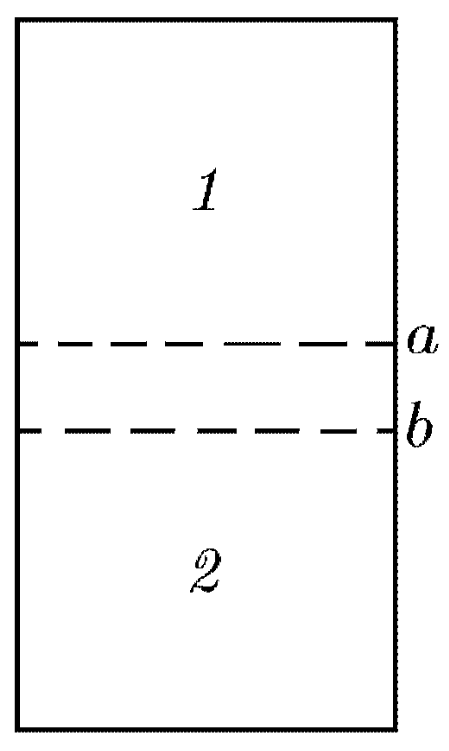
\includegraphics[width=30mm]{ris31.png}	
\end{wrapfigure}
 Таким образом мы квазистатически смешаем 2 газа и 
\begin{equation}
\label{eq:entrop}
 \Delta S=\Delta S_1 + \Delta S_2=R\left(\nu_1 \ln \frac{V}{V_1}+\nu_2\ln \frac{V}{V_2}\right)>0
 \end{equation}
 Но если же газы тождественны ($\nu_1=\nu_2=\nu/2;\ V_1=V_2=V/2$), то по формуле $\Delta S=\nu R \ln 2$, однако конечное состояние макроскопически ничем не отличается от начального. Энтропия возросла, а состояние системы не изменилось. В этом и есть \textbf{парадокс Гиббса.}\\
 \eqref{eq:entrop} выведена для случая смешивания существенно различных газов. Для тождественных газов рассуждения неприменимы. Принципиально невозможно квазистическок перемешивание тождественных газов вышеописанным способом.